\documentclass[12pt]{article}

\title{Developement of a neural network from scratch in C++/CUDA for particle tracking}
\author{Simone Balducci}
\date{}

\usepackage{amsmath}
\usepackage{amsfonts}
\usepackage{amssymb}
\usepackage{amsthm}
\usepackage{bbold}
\usepackage[margin=2cm]{geometry}
\usepackage{pgfplots}
\usepackage{fancyhdr}
\usepackage{physics}
\usepackage{systeme,mathtools}
\usepackage{graphicx}
\usepackage{float}
\usepackage{relsize}
\usepackage{dsfont}
\usepackage{calligra}
\usepackage{float}
\usepackage[utf8]{inputenc}
\usepackage{listings}
\usepackage{xcolor}

\definecolor{codegreen}{rgb}{0,0.6,0}
\definecolor{codegray}{rgb}{0.5,0.5,0.5}
\definecolor{codepurple}{rgb}{0.58,0,0.82}
\definecolor{backcolour}{rgb}{0.95,0.95,0.92}

\lstdefinestyle{mystyle}{
    backgroundcolor=\color{backcolour},   
    commentstyle=\color{codegreen},
    keywordstyle=\color{blue},
    numberstyle=\tiny\color{codegray},
    stringstyle=\color{codepurple},
    basicstyle=\ttfamily\footnotesize,
    breakatwhitespace=false,         
    breaklines=true,                 
    captionpos=b,                    
    keepspaces=true,                 
    numbers=left,                    
    numbersep=5pt,                  
    showspaces=false,                
    showstringspaces=false,
    showtabs=false,                  
    tabsize=2
}

\lstset{style=mystyle}


\newcommand{\vv}{\vec{v}}
\newcommand{\vw}{\vec{w}}
\newcommand{\vx}{\vec{x}}
\newcommand{\R}{\Re}
\newcommand{\la}{\lambda}
\newcommand{\lang}{\left\langle}
\newcommand{\rang}{\right\rangle}
\newcommand{\lbra}{\left\lbrace}
\newcommand{\rbra}{\right\rbrace}
\newcommand{\ih}{\hat{i}}
\newcommand{\jh}{\hat{j}}
\newcommand{\kh}{\hat{k}}
\newcommand{\nnabla}{\vec{\nabla}}
\newcommand{\rita}{\rightarrow}

\begin{document}
\maketitle

\section{Physical background}
\subsection{Review of special relativity}
The most fundamental equation in special relativity defines the 4-momentum of a particle:
\begin{equation}
  E^2 = p^2c^2 + m^2c^4
\label{fundamental}
\end{equation}
where $E$ is the energy of the particle, $p$ is its momentum, $m$ is the rest mass and $c$ is the speed of light. \\
In particle physics usually the following units are used:
\begin{itemize}
  \item Energy is measured in $GeV$, where $1\,eV$ is the energy acquired by an electron accelerated by an
	electric potential of $1\,V$ over a distance of $1\,m$.
  \item Momentum is measured in $GeV/c$
  \item Mass is measured in $GeV/c^2$
\end{itemize}
It should be noted that usually, for convenience, the units of mass, momentum and energy are all indicated 
simply as $GeV$. \\
When using this units, Eq. \ref{fundamental} assumes the convenient form:
\begin{equation}
  E^2 = p^2 + m^2
  \label{fundamental_conv}
\end{equation}
The relativistic momentum is defined as:
\begin{equation}
  p = \gamma m v
\end{equation}
where $\gamma m$ is the relativistic mass, and $\gamma$ is a unitless constant known as the lorentz factor
and defined as:
\begin{equation}
  \gamma = \frac{1}{\sqrt{1 - \beta^2}}
\end{equation}
where beta is $v/c$. \\
The kinematics of a particle is fully defined by the combination of its energy and the three components
of its momentum. This four quantities are known as the 4-momentum of the particle. \\ \\
The rest mass of a particle is an intrinsic property of a particle. To measure the mass of a particle we
need the 4-momenta of its products. \\
If a particle $H$ decays in two generic particles $A$ and $B$, by the conservation of energy and momentum
we can write:
\begin{equation}
	E_H = E_A + E_B \hspace{2cm} \vec{p}_H = \vec{p}_A + \vec{p}_B
\end{equation}
The 4-momenta of both $A$ and $B$ are measured in the detector, which means that we can calculate the mass
of $H$ as:
\begin{equation}
  m_H = \sqrt{E^2_H - p^2_H}
\end{equation}
This quantity is called invariant mass, because it is always the same for all the possible combinations of
$E_H$ and $p_H$, at least in an ideal detector.

\subsection{Review of particle physics}
\begin{figure}
  \centering
  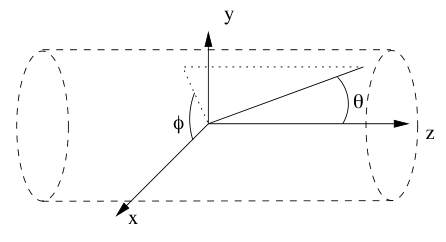
\includegraphics[scale=0.8]{img/atlas_frame.png}
  \caption{Reference frame used in the ATLAS experiment}
\end{figure}
In the conventional 3D reference frame used in the ATLAS experiment, the $z$ axis points along the horizontal 
beam line and the $x$ and $y$ axes are in the transverse plate, with the $y$ axis pointing towards the top 
of the detector. The angle $\theta$ is the polar angle and $\phi$ is the azimuthal angle. \\
Transverse quantities (mass, momentum and energy) are defined as projections on the $x-y$ plane. \\
Usually, instead of the polar angle $\theta$ it is useful to use the pseudorapidity $\eta$, which is defined
as:
\begin{equation}
  \eta = -\log \tan(\frac{\theta}{2})
\end{equation}
A pseudorapidity $\eta=0$ corresponds to a particle moving on the $x-y$ plane, whereas $\eta=\pm\infty$
corresponds to a particle traversing along the $z$ axis. \\
A practical difficulty is that many particles are lost in the direction of the $z$ axis, which means that we 
can count on conservation laws only on the transverse plane, thus the importance of defining transverse 
quantities. \\ \\
Now that we have described the spatial and angular coordinates used in this kind of experiments, we can 
define some other important quantities. \\
The components of momentum can be written as:
\begin{equation}
  \vec{p} = \begin{pmatrix}
	p_x \\
	p_y \\
	p_z
  \end{pmatrix} = \begin{pmatrix}
	p_T\cos\phi \\
	p_T\sin\phi \\
	p_T\sinh\eta
  \end{pmatrix}
\end{equation}
where $p_T$ is the transverse momentum, defined as
\begin{equation}
  p_T = \sqrt{p_x^2 + p_y^2}
\end{equation}
The missing transverse energy, $\vec{E}^{miss}_{T}$ is a two dimensional vector defined as:
\begin{equation}
  \vec{E}^{miss}_{T} = \begin{pmatrix}
	|\vec{E}^{miss}_{T}| \cos\phi_T \\
	|\vec{E}^{miss}_{T}| \sin\phi_T
  \end{pmatrix}
\end{equation}
where $\phi_T$ is the azimuthal angle of the missing transverse energy. \\
The invariant mass $m_{inv}$ of two particles is the invariant mass of the sum of the two 4-momenta, and 
the transverse mass $m_{tr}$ is the invariant mass of the sum of the two 4-momenta setting the $z$ component 
to zero, thus only keeping the transverse components.
So if $\vec{a}$ and $\vec{b}$ are the 4-momenta of two particles $A$ and $B$, $m_{inv}(\vec{a},\vec{b})$ 
and $m_{tr}(\vec{a},\vec{b})$, neglecting the two rest masses, are defined as:
\begin{equation}
  m_{inv}(\vec{a},\vec{b}) = \sqrt{\left(\sqrt{a_x^2 + a_y^2 + a_z^2} + \sqrt{b_x^2 + b_y^2 + b_z^2}\right)^2 
  - (a_x^2 + b_x^2)^2 - (a_y^2 + b_y^2)^2 - (a_z^2 + b_z^2)^2}
\end{equation}
\begin{equation}
  m_{tr}(\vec{a},\vec{b}) = \sqrt{\left(\sqrt{a_x^2 + a_y^2} + \sqrt{b_x^2 + b_y^2}\right)^2 
  - (a_x^2 + b_x^2)^2 - (a_y^2 + b_y^2)^2}
\end{equation}
The pseudorapidity separation between two particles $A$ and $B$ is defined as:
\begin{equation}
  |\eta_A - \eta_B|
\end{equation}
and their R separation is:
\begin{equation}
  \sqrt{(\eta_A - \eta_B)^2 + (\phi_A - \phi_B)^2}
\end{equation}

\subsection{Description of the dataset and goal of the project}
The Higgs boson dacays into two taus leptons. This process theoretically interesting, becuase the Higgs 
boson is the particle responsible for the mass of the other elementary particles, but it is an experimentally 
challenging one. This difficulty is due to two reasons:
\begin{itemize}
  \item The neutrinos are not measured in the detector, so their presence in the final state makes it 
	difficult to evaluate the mass of the Higgs candidate
  \item The $Z$ boson can also decay in two tau leptons, and this process happens much more frequently than 
	the decay of the Higgs boson. Furthermore, since the mass of the $Z$ and $H$ bosons are very similar (
	respectively $91\,GeV$ and $125\,GeV$), the two events are very difficult to separate.
\end{itemize}

The simulated data contains signal and background events. The signal events are those in which Higgs bosons
are produced. The background events are generated by other well known processes which can produce events with 
at least one electron or muon and a hadronic tau, thus mimicking the signal. For simplicity, only three
background processes are used:
\begin{itemize}
  \item Decay of $Z$ boson into two taus
  \item Decay of a pair of $top$ quarks into a lepton and a hadronic tau
  \item Decay of the $W$ boson into an electron or muon and a hadronic tau
\end{itemize}
The particles and pseudo-particles of interest in this case are electrons, muons, hadronic tau, jets and 
missing transverse energy. \\
Electrons, muons and hadronic tau are the three leptons. Electrons and muons live long enough to reach the 
detector, so their 4-momenta can be measured directly. Taus, on the other hand, decay almost immediately 
into either an electron and two neutrinos, a muon and two neutrinos or a charged particles and a neutrino. \\
Jets are pseudo particles that originate from a high energy quark or gluon, and they appear in the detector 
as collimated energy deposits.

\section{Implementation of the neural network framework}
Here is described the errorb backpropagation algorithm, which is used for training the neural network. \\
After that, there is a description of the code which constructed the neural network framework used in the 
project. 
\subsection{Description of the error backpropagation algorithm}
We derive the backpropagation algorithm for a general network having a feed-forward topology, an 
arbitrary differentiable non-linear activation function and a class of error functions. \\
In a feed-forward network we have that each unit computes a weighted sum of its inputs as:
\begin{equation}
  a_j = \sum_i w_{ji}z_i
\end{equation}
where $z_i$ is the activated input. \\
The terms $a_j$ are then passed inside the activation function $h(\cdot)$, resulting in:
\begin{equation}
  z_j = h(a_j)
\end{equation}
Here $z_j$ could be the outputs of the network and $a_j$ could be the input. \\
This process is called \textit{forward propagation}, because there is a forward-directed flow of
information inside the network. \\
Now, to adjust the weights $w_{ji}$ we need to calculate the gradient of the terms of the error  
function, $E_n$. Since the value of the error only depends on the weights through terms $a_j$, we 
can use the chain rule:
\begin{equation}
  \frac{\partial E_n}{\partial w_{ji}} = 
  \frac{\partial E_n}{\partial a_{j}}\frac{\partial a_j}{\partial w_{ji}}
\end{equation}
where we see that the second derivative is simply $z_i$, and we call the first term $\delta_j$
\begin{equation}
  \delta_j = \frac{\partial E_n}{\partial a_j}
\end{equation}
So we thus obtain the simple equation:
\begin{equation}
  \frac{\partial E_n}{\partial w_{ji}} = \delta_j z_i
  \label{loss_gradient_weight}
\end{equation}
This means that the problem of calculating the gradient of the error function boils down to
calculating $\delta_j$. \\
For the output layer it's trivial to calculate $\delta_j$, since it's simply:
\begin{equation}
  \delta_j = y_j - t_j
  \label{output_delta}
\end{equation}
where $t_j$ are the labels given in the training data. \\
For the hidden layers we use again the chain rule:
\begin{equation}
  \delta_j = \frac{\partial E_n}{\partial a_j}
  = \sum_k \frac{\partial E_n}{\partial a_k}\frac{\partial a_k}{\partial a_j}
  \label{hidden_layers_delta}
\end{equation}
where $\partial E_n / \partial a_k = \delta_k$ and $\partial a_k / \partial a_j = h'(a_j)w_{kj}$
so we obtain:
\begin{equation}
  \delta_j = h'(a_j)\sum_k w_{kj}\delta_k
  \label{simplified_hidden_layer_delta}
\end{equation}
So we see that the value of $\delta$ for a particular hidden unit can be obtained by propagating backwards the $\delta$ values from layers higher up in the network.

\subsection{Constructing the activation functions}
The choice of the activation function is of the highest importance when working with neural networks. \\
It is very convenient to write the activation functions as functors, instead of normal functions. This is
convinient because then the activation function can be passed to the neural network as a template parameter,
thus making it known at compile time. \\
A functor is an object that behaves like a function. In $C++$, functors are defined by declaring a struct 
and providing an operload for the $operator()$. These structs must be templated on the type of the data
contained in the neurons of the neural network. \\
As an example, below is reported the code of the most common and widely used activation function, the sigmoid
function, which is mathematically defined as:
\begin{equation}
  S(x) = \frac{1}{1 + e^{-x}}
\end{equation}
with derivative:
$$
  S'(x) = \frac{e^{-x}}{(1 + e^{-x})^2} = \frac{e^{-x}}{1 + e^{-x}}\frac{1}{1 + e^{-x}} 
  = S(x)\left(1 - S(x)\right)
$$
so:
\begin{equation}
  S'(x) = S(x)\left(1 - S(x)\right)
\end{equation}

\begin{lstlisting}[language=C++]
template <typename T>
struct Sigmoid {
  double operator()(double x) { return 1. / (1 + std::exp(-x)); }

  std::vector<T> operator()(const std::vector<T>& vec) {
	size_t N{vec.size()};
	std::vector<T> activated(N);
	for (int i{}; i < N; ++i) {
	  activated[i] = Sigmoid<T>()(vec[i]);
	}
	
	return activated;
  }

  template <typename E>
  std::vector<T> operator()(const std::vector<E>& vec) {
	size_t N{vec.size()};
	std::vector<T> activated(N);
	for (int i{}; i < N; ++i) {
	  activated[i] = Sigmoid<T>()(static_cast<T>(vec[i]));
	}
	
	return activated;
  }

  // Derivative of the activation function
  double grad(double activated_value) {
	return activated_value * (1 - activated_value);
  }
  std::vector<double> grad(shared<Layer<T>> layer) {
	int N{layer->size()};
	std::vector<double> gradient_values(N);
	for (int i{}; i < N; ++i) {
	  gradient_values[i] = grad((*layer)[i]);
	}

	return gradient_values;
  }
  std::vector<double> grad(std::vector<T> node_values) {
	int N{node_values.size()};
	std::vector<double> gradient_values(N);
	for (int i{}; i < N; ++i) {
	  gradient_values[i] = grad(node_values[i]);
	}

	return gradient_values;
  }
};
\end{lstlisting}
In addition to the overloads of the $operator()$, it is necessary to provide one or more methods calculating
the gradient of the sigmoid for a particular value. \\ \\
In addition to the sigmoid, other activation functions have been implemented and added to the framework. \\
Here is a list of all the activators present in the framework:
\begin{itemize}
  \item Step function
  \item Linear function
  \item Sigmoid 
  \item Hyperbolic tangent
  \item Elu
  \item Leaky ReLU
  \item Parametric ReLU
  \item Swish
  $$
	Swish(x) = \frac{x}{1 + e^{-x}} = x S(x)
  $$	
\end{itemize}

\subsection{Constructing the loss functions}
As it's been shown in the section regarding the backpropagation algorithm, during the training phase of the
network, after each entry of the dataset the weights are adjusted using the gradient of a function called 
the loss function. \\
For the same reasons of the activation functions, the loss functions are also defined as functors, for which 
are also provided methods that calculates the gradient. Considering the relation contained in Eq. 
\ref{hidden_layers_delta}, it is convenient to define the gradient methods of the functors so that they 
return the gradient of the loss function with respect to the activated node values. \\
For what concerns the structure of the functors, just like the activators, they must be templated on the 
data type of the neurons, but they also need two more template parameters, one for the data type of the 
weights $w_{ij}$ and one for the activation function. The last template parameter is needed because, as 
can be seen in Eq. \ref{simplified_hidden_layer_delta}, one of the factors used when calculating the gradient
of the loss is the gradint of the activation function. \\
The most popular loss function is the mean squared error, defined as:
\begin{equation}
  E(\vec{y}) = \frac{1}{2}\sum_k (y_k - t_k)^2
\end{equation}
where $y_k$ are the output neurons of the network and $t_k$ are the targets of the respective neurons. \\
Below is reported the code for the mean squared error functor:
\begin{lstlisting}[language=C++]
template <typename T, typename W, template <typename E> typename Activator>
struct MeanSquaredError {
  double operator()(const std::vector<T>& node_values, const std::vector<T>& expected_values) {
    double error{};
    int N{node_values.size()};
    for (int node_index{}; node_index < N; ++node_index) {
      error += pow(node_values[node_index] - expected_values[node_index], 2);
    }
    error /= N;

    return error;
  }

  // Derivative of the error function with respect to the activated node values
  template <typename U>
  std::vector<double> grad(const std::vector<U>& expected_values,
                           int layer_id,
                           const std::vector<shared<Layer<T>>>& layers,
                           const std::vector<shared<Matrix<W>>>& weights) {
    if (layers[layer_id + 1] == nullptr) {
      int N{layers[layer_id]->size()};
      std::vector<double> delta(N);
      for (int node_index{}; node_index < N; ++node_index) {
        delta[node_index] = (*layers[layer_id])[node_index] - static_cast<T>(expected_values[node_index]);
      }

      return delta;
    } else {
      Activator<T> act;
      int N{layers[layer_id]->size()};
      std::vector<double> delta(N);

      for (int node_index{}; node_index < N; ++node_index) {
        std::vector<double> previous_delta{grad(expected_values, layer_id + 1, layers, weights)};
        delta[node_index] =
            act.grad((*layers[layer_id])[node_index]) * (weights[layer_id]->transpose() * previous_delta)[node_index];
      }

      return delta;
    }
  }
};
\end{lstlisting}

\subsection{Constructing the layer class}
The layer class is a simple class template, templated on the type of the neuron data, with said data being 
stored in a vector.

\subsection{Constructing the neural network class}
Now that we have defined the functors for the activation functions and the loss functions, we can move on to
writing the class for the neural network. \\
The class needs four template parameters:
\begin{itemize}
  \item One for the type of the neuron data
  \item One for the type of the weights
  \item One template template parameter for the activation function
  \item One template template template parameter for the loss function
\end{itemize}
\begin{lstlisting}[language=C++]
template <typename T,
          typename W,
          template <typename F> typename Activator,
          template <typename E, 
					typename LW, 
					template <typename K> typename Act> typename Loss>
class Network {
private:
  int n_layers;
  std::vector<shared<Layer<T>>> m_layers;
  std::vector<shared<Matrix<W>>> m_weights;
  std::vector<shared<std::vector<W>>> m_bias;
\end{lstlisting}
The attributes of this class are:
\begin{itemize}
  \item $n\_layers$, an integer representing the number of layers, including the input and output layer
  \item $m\_layers$, a vector containing shared pointers pointing to layers
  \item $m\_weights$, a vector containing shared pointers pointing to the weight matrices
  \item $m\_bias$, a vector containing shared pointers pointing to vectors representing the bias
\end{itemize}
After the usual constructors, getters and setters, the methods for the training of the network are defined. \\
The method $train$ calls the methods for the forward propagation and the backpropagation. The forward 
propagation simply consists of calculating the data values for the following layer by doing the matrix-vector 
product of the weight matrix with the layer vector, and then applying the activation function to the 
resulting layer.
\begin{lstlisting}[language=C++]
std::vector<T> forward_propatation(shared<Layer<T>> layer,
																	 shared<Matrix<W>> weight_matrix,
																	 shared<std::vector<W>> bias_vector) {
  std::vector<W> next_layer_nodes{*weight_matrix * layer->nodes() 
									+ *bias_vector};

  return Activator<T>()(next_layer_nodes);
}

void forward_propatation() {
  for (int i{}; i < n_layers - 1; ++i) {
    std::vector<T> new_layer_data{forward_propatation(m_layers[i],
																										  m_weights[i],
																										  m_bias[i])};
    m_layers[i + 1]->set_node_data(new_layer_data);
  }
}
\end{lstlisting}
After the forward propagation we use the backpropagation to update the weights of the network. To do this we
have to apply the Eq. \ref{loss_gradient_weight}, \ref{output_delta}, \ref{simplified_hidden_layer_delta}.
\begin{lstlisting}[language=C++]
void back_propagation(const std::vector<U>& target, int layer_id, double eta) {
  Loss<T, W, Activator> loss_function;
  Matrix<W> loss_grad(loss_function.grad(target, layer_id + 1, m_layers, m_weights));
  Matrix<T> activated_values_grad(m_layers[layer_id]->nodes());
  *m_weights[layer_id] -= eta * (loss_grad * activated_values_grad.transpose());
  *m_bias[layer_id] -= eta * loss_grad;
}

void back_propagation(double eta, const std::vector<U>& target) {
  for (int layer_id{n_layers - 2}; layer_id >= 0; --layer_id) {
    back_propagation(target, layer_id, eta);
  }
}
\end{lstlisting}
The main is that when calculating the gradient of the loss we must differentiate between output and hidden 
layers. This is done by adding an additional $nullptr$ to $m\_layers$ , so that if the pointer corresponding
to the next layer is null, the current layer is the output layer, otherwise it's an hidden layer.

\end{document}
